\documentclass[a4paper,12pt]{article}
\usepackage{amsmath}
\usepackage{url}
\usepackage{amssymb}
\usepackage{graphicx}
%\documentclass{article}
\usepackage{setspace, enumitem,titlesec}
\usepackage{calc}
			% Activate to display a given date or no date
\usepackage{mathtools}
\usepackage{mathrsfs }
\DeclarePairedDelimiter\ceil{\lceil}{\rceil}
\DeclarePairedDelimiter\floor{\lfloor}{\rfloor}
\usepackage{algorithm}
\usepackage{algorithmic}
\usepackage{fancybox}
\usepackage{array, makecell} %
\usepackage{amsmath}
\usepackage{amssymb}
\usepackage{amsthm}
\usepackage{cite}
\usepackage{authblk}
\usepackage{multirow}% http://ctan.org/pkg/multirow
\usepackage{hhline}% http://ctan.org/pkg/hhline
%\usepackage{algpseudocode}

\usepackage{hyperref}


%\renewcommand{\thepseudonum}{\roman{pseudonum}}
\renewcommand\labelenumi{(\theenumi)}
%vector
\renewcommand{\vec}[1]{\mathbf{#1}}
\title {Segment Point Cloud by Using Sequential Labeling and RANSAC Algorithms }
%\author{jim.morris.shen@gmail.com}
%\author{The Graduate Center, City University of New York}
\author{Xiaoke Shen}
\affil{The Graduate Center, City University of New York}
\date{}
\begin{document}
\maketitle
\begin{abstract}
This report is the submission of the project 1 of the 3d computer vision course provided by the Graduate Center of CUNY. The project is required to do the segmentation based on the raw cloud point data. Sequential labelling and RANSAC algorithms are used to explore the different segmentation results. The code of this project is shared on github: \url{https://github.com/liketheflower/3d_vision.git}

\end{abstract}


%\textbf{Due Mar 1st 11:59 pm. 10 points for each exercise and 20 points for the extra credit exercise }\\
\section{Project description}
One of the earlier stages in range image analysis is segmentation. The input to this
module is a range image acquired from a specified viewpoint. This range image is
expressed as a two-dimensional array of 3-D points. 3-D points that are neighbors in this
array are probably neighbors in the actual 3-D surface, unless the points lie on a shape
discontinuity. Each 3-D point is expressed with four coordinates. The first three are the
Cartesian $x, y, z$ coordinates expressed in the local coordinate system of the range scan.
The fourth is a number that encodes the power of the returned laser beam.\\
The segmentation module groups 3-D points that are part of the same surface by giving
them the same label. One way to do this is to override the fourth coordinate of each point
with the point?s label.\\
Given a range image R acquired from one particular viewpoint segment this image into
planar components. Visualize the result by displaying each segment (i.e. set of points that
lie on the same surface) with different colors.
Test the following algorithms:\\

(a) Compute normals for all points and apply a region-growing algorithm using the grid structure of the range images.
(b) Apply a RANSAC algorithm by selecting 3 points to define a plane and then score it.
(c) Apply a RANSAC algorithm by selecting 1 point and its normal to define a plane.

\section{Submissions}
\subsection{Original cloud point data visualization}
\begin{figure}[H]
  \begin{center}
      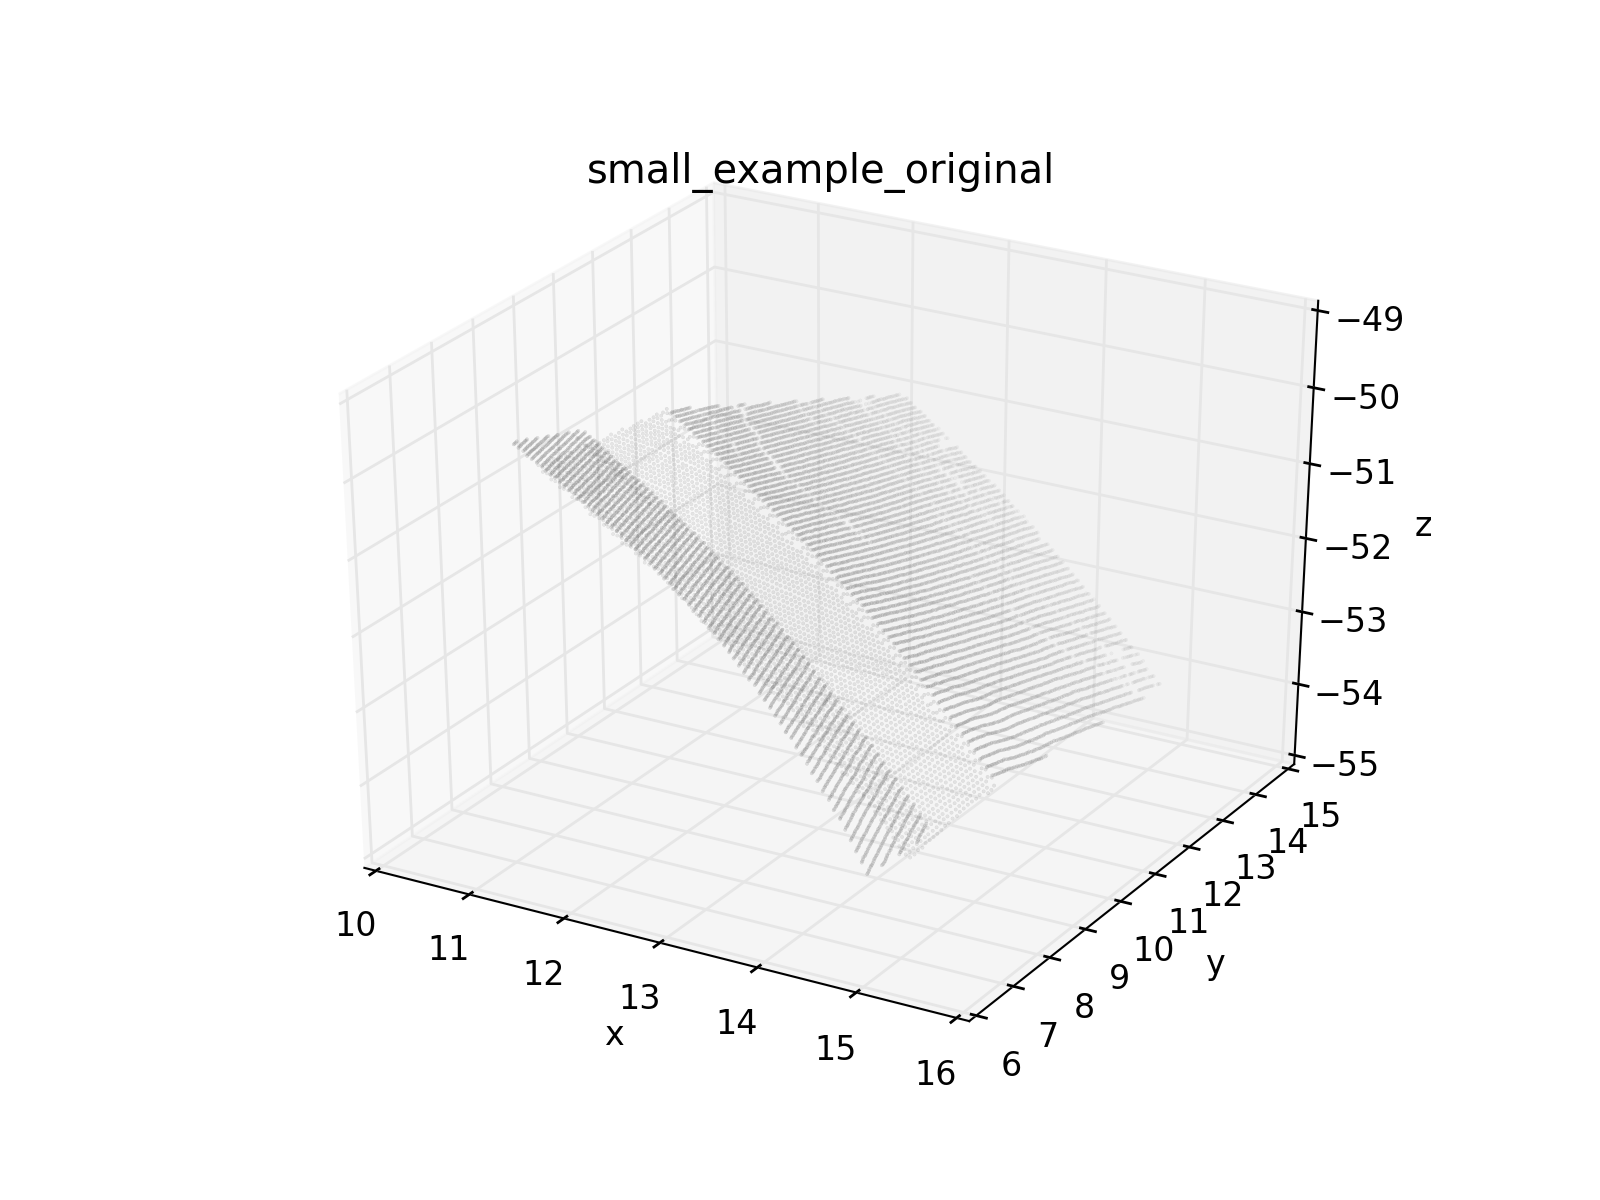
\includegraphics[scale=0.65]{small_example_original.png}
\end{center}
\caption{The original point cloud of the small example.}
 \label{fig:sml_origin}
 \end{figure}
 
  \begin{figure}[H]
  \begin{center}
      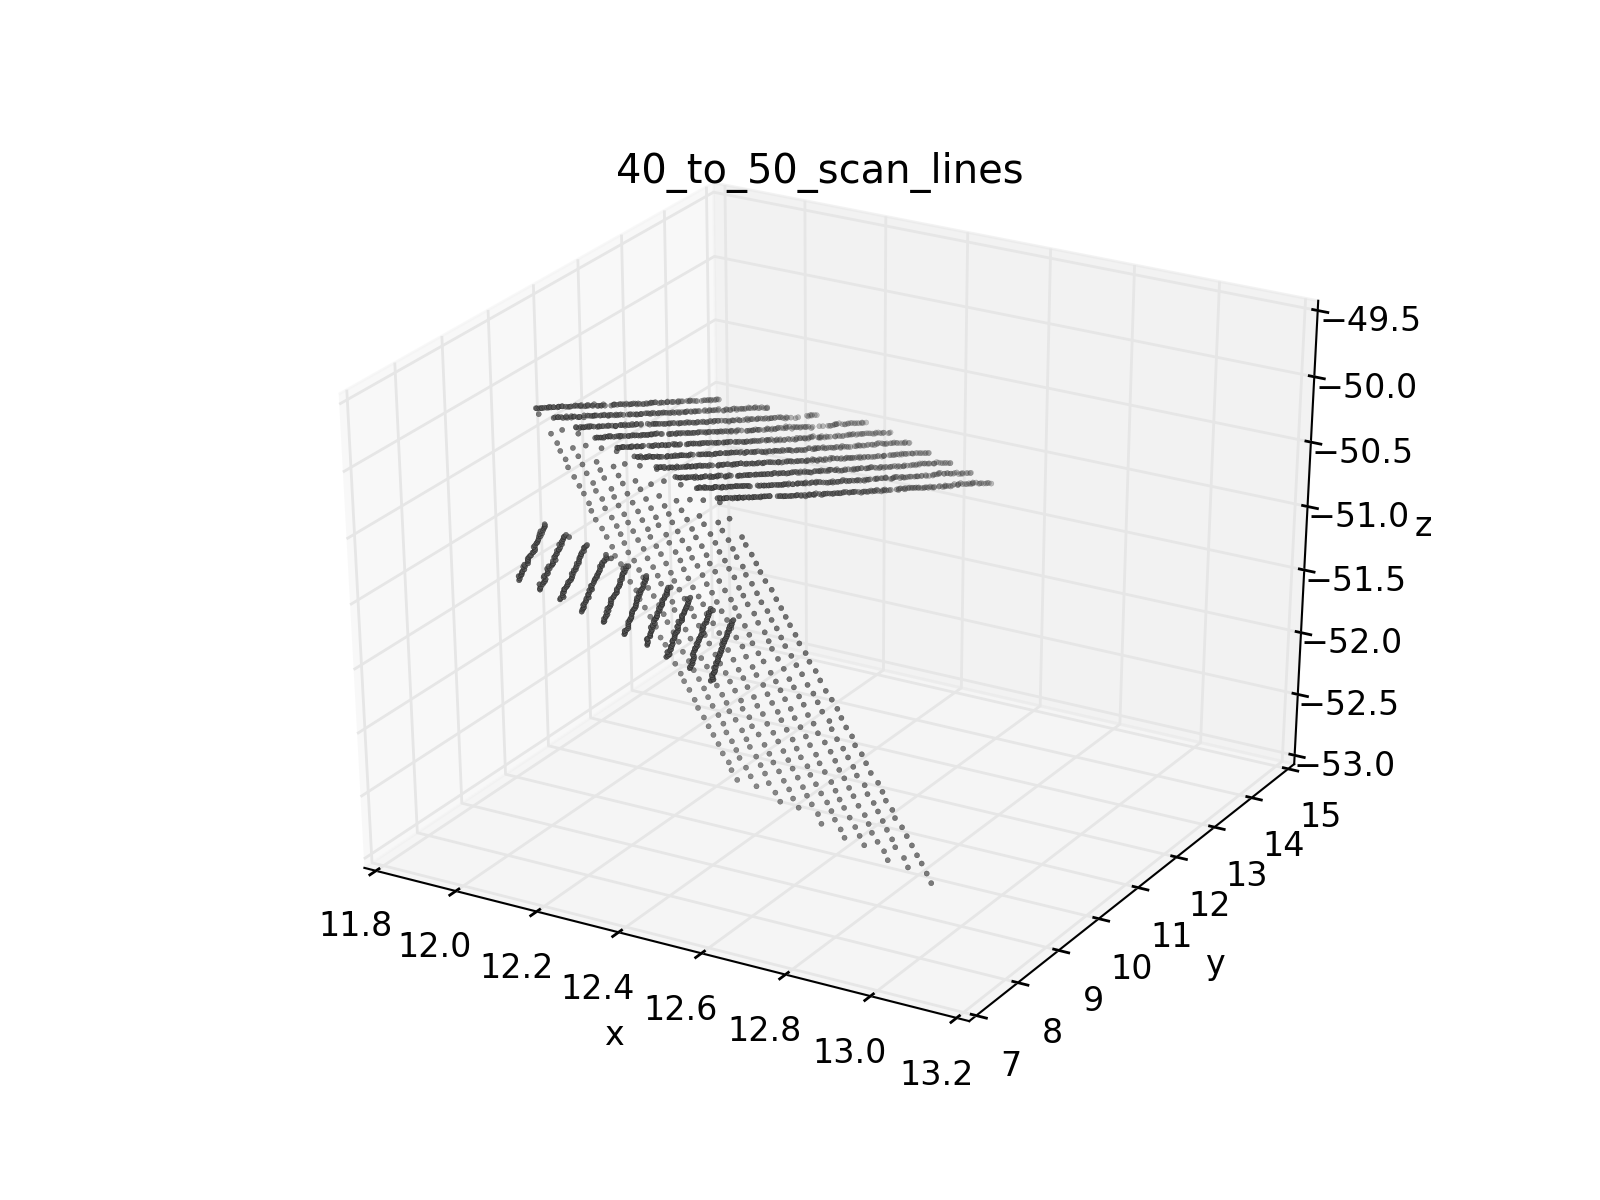
\includegraphics[scale=0.65]{40_to_50_scan_lines.png}
\end{center}
\caption{The 40 to 50 scan line of the point cloud of small example.}
 \label{fig:40_50_sml_origin}
 \end{figure}

  \begin{figure}[H]
  \begin{center}
      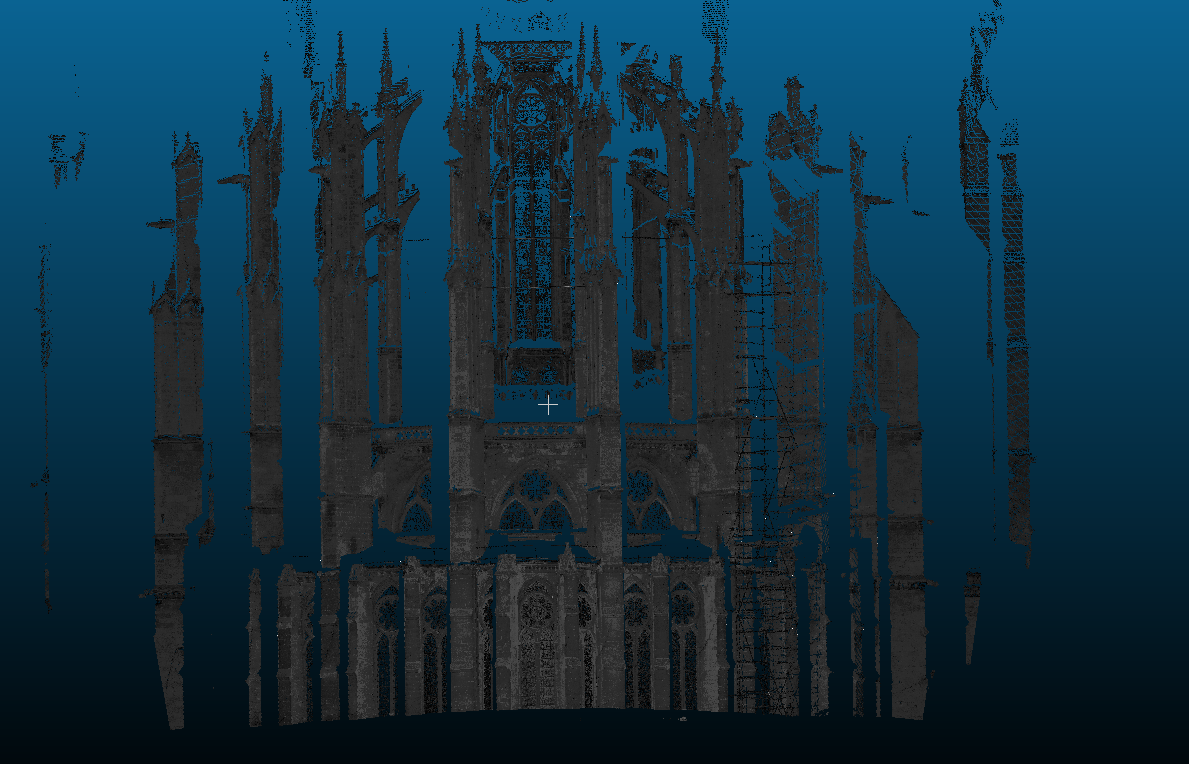
\includegraphics[scale=0.4]{big_example.png}
\end{center}
\caption{The point cloud of big example.}
 \label{fig:big}
 \end{figure}
\subsection{Submission of part (a)}


%40_to_50_scan_lines.png
%big_example.png
%hist_of_abs_norm.png
%norm_map_big.png
%number_ptx_per_label.png
%small_example_seq_b.png

 \begin{figure}[H]
  \begin{center}
      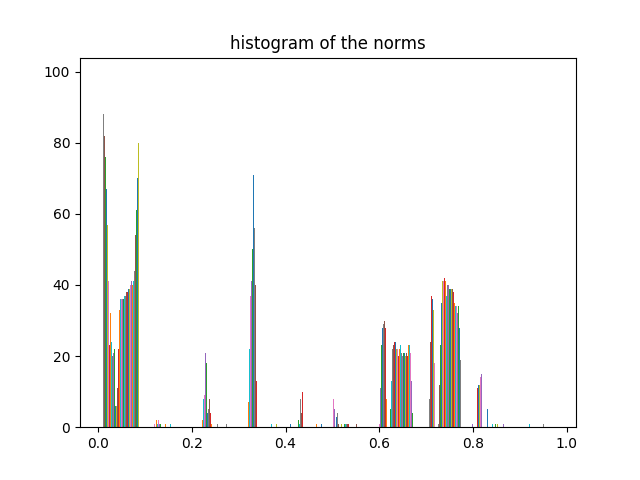
\includegraphics[scale=0.6]{hist_of_abs_norm.png}
\end{center}
\caption{The original point cloud of the small example.}
 \label{fig:sml_origin}
 \end{figure}
 
  \begin{figure}[H]
  \begin{center}
      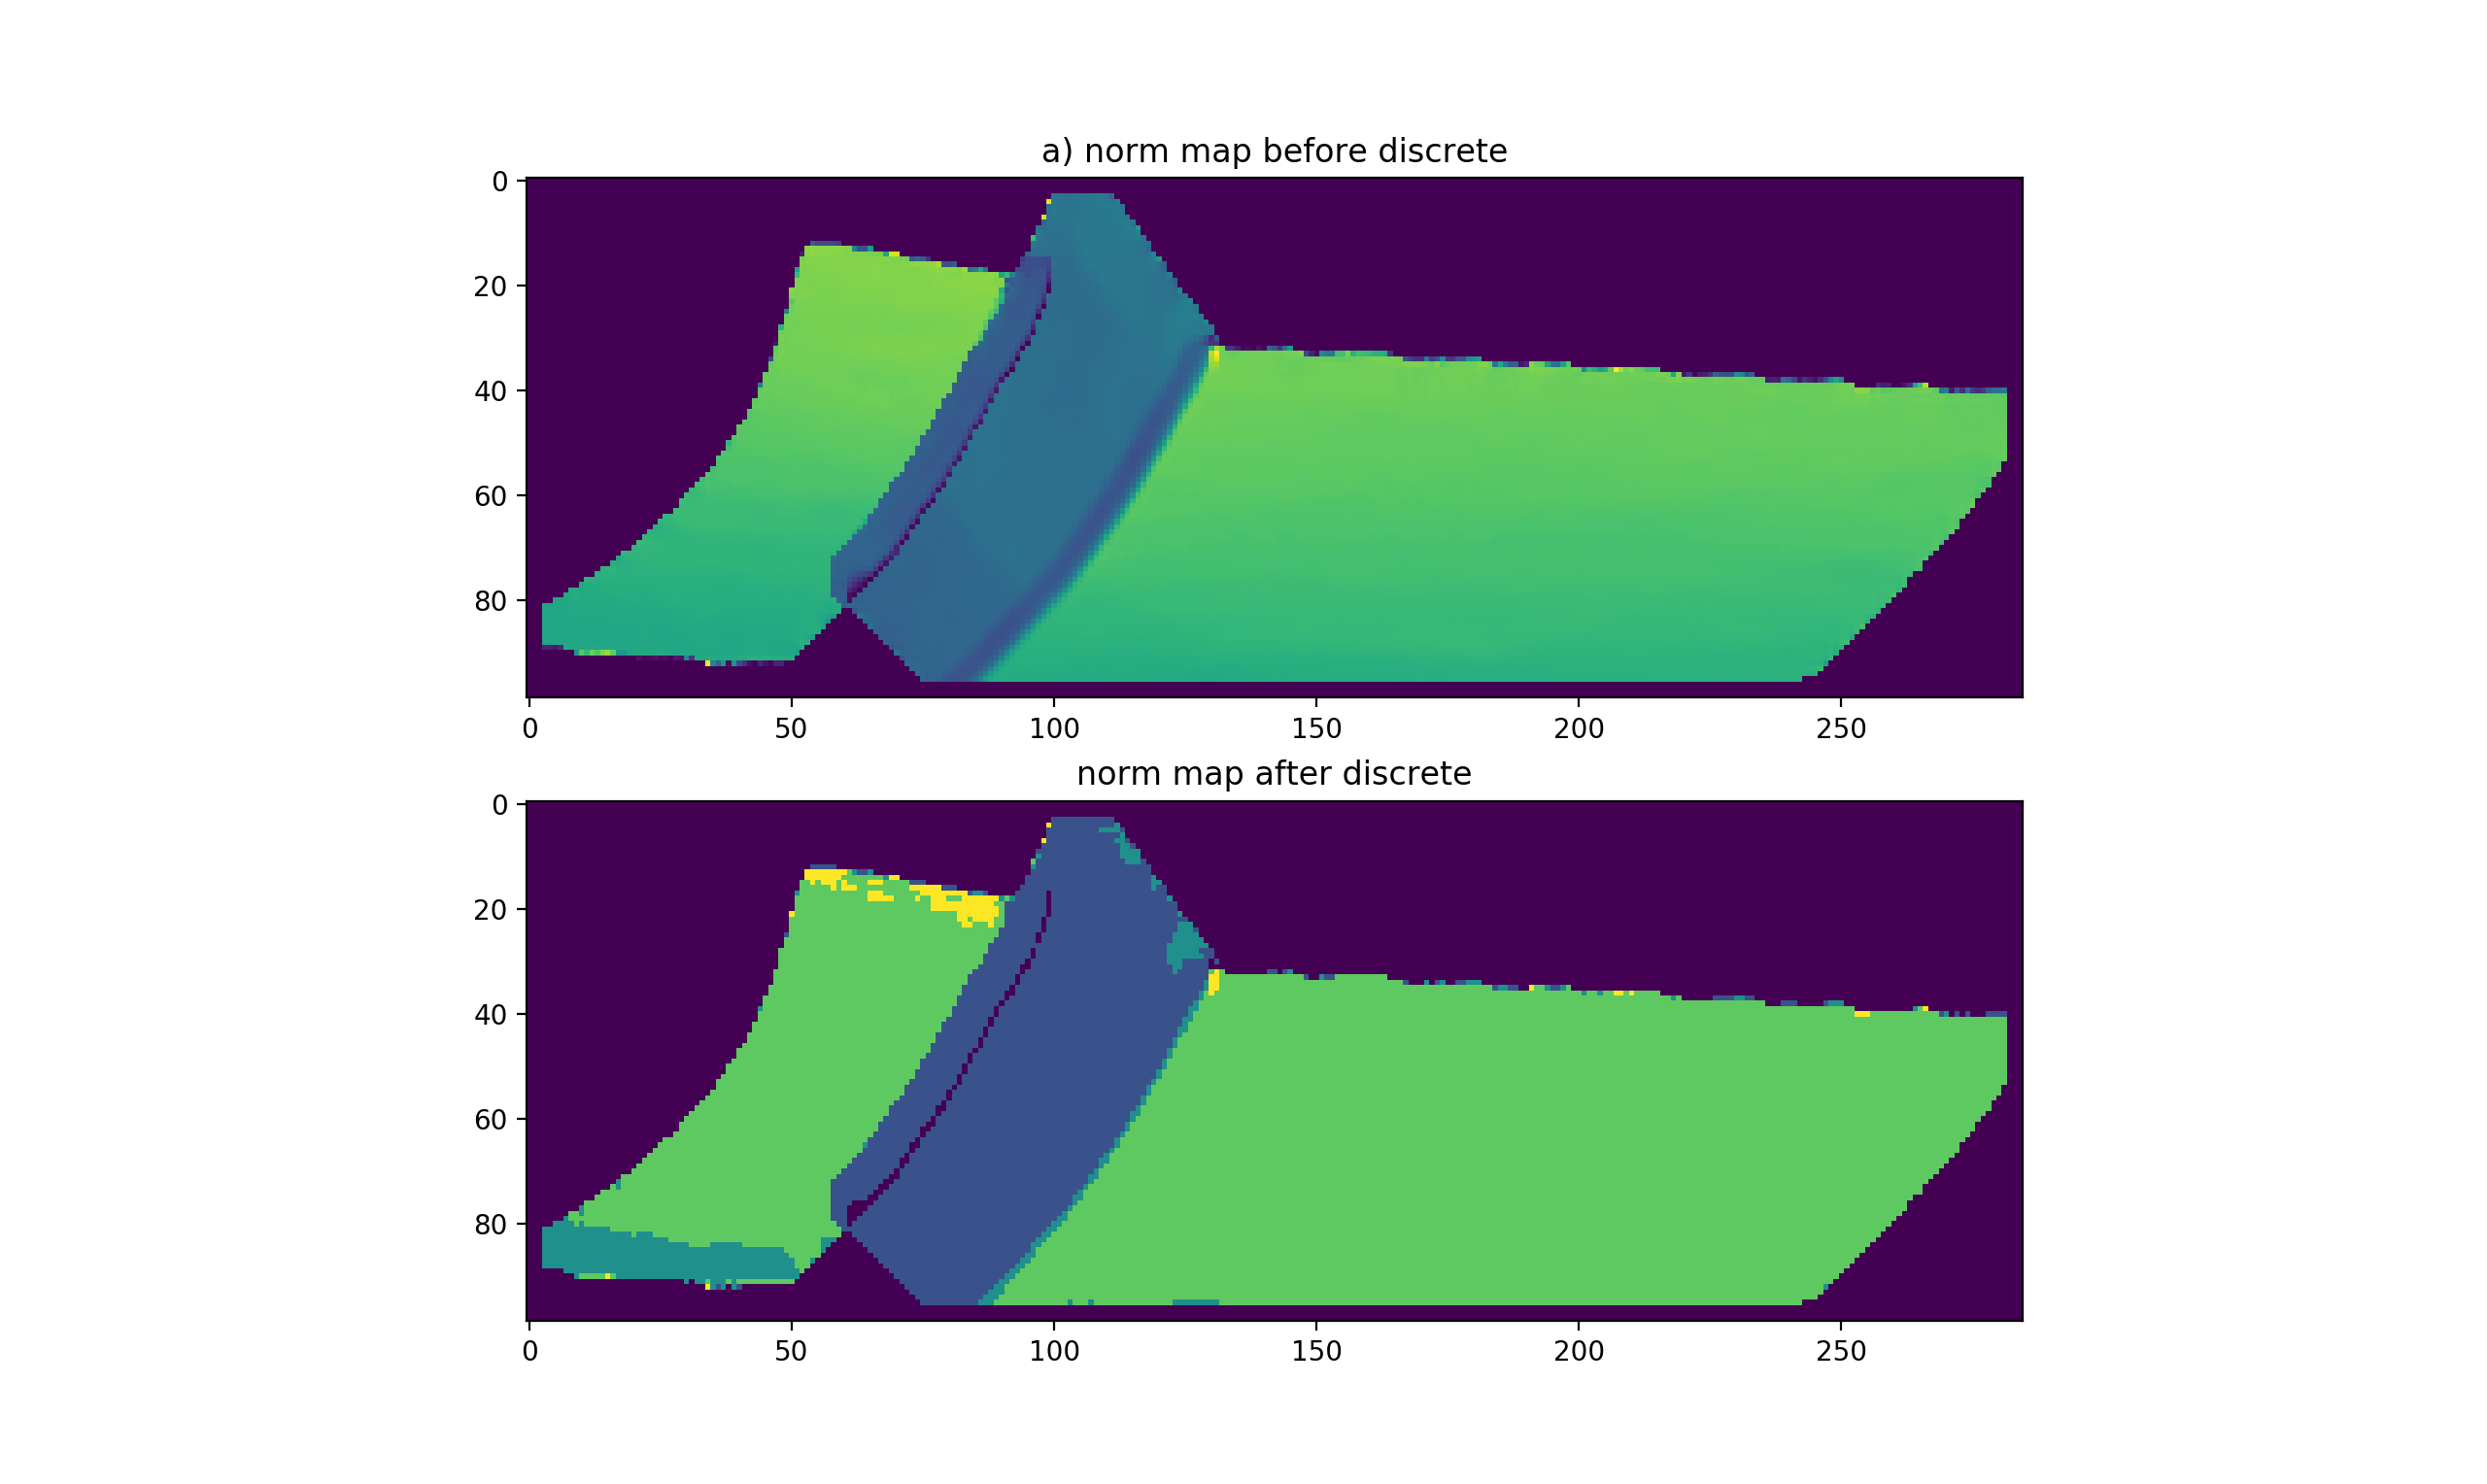
\includegraphics[scale=0.5]{norm_map_big.png}
\end{center}
\caption{The 40 to 50 scan line of the point cloud of small example.}
 \label{fig:40_50_sml_origin}
 \end{figure}
 
 
   \begin{figure}[H]
  \begin{center}
      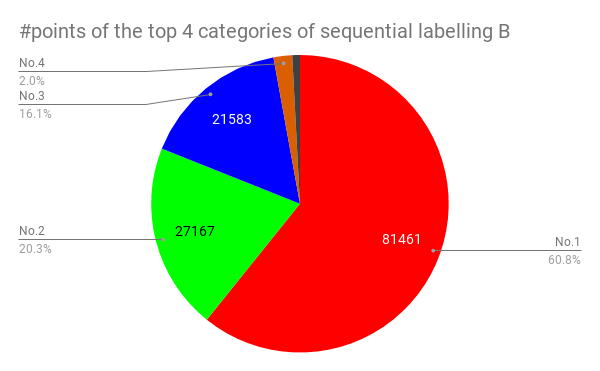
\includegraphics[scale=0.6]{label_statis_seq_b.png}
\end{center}
\caption{The 40 to 50 scan line of the point cloud of small example.}
 \label{fig:40_50_sml_origin}
 \end{figure}
 
 
 
   \begin{figure}[H]
  \begin{center}
      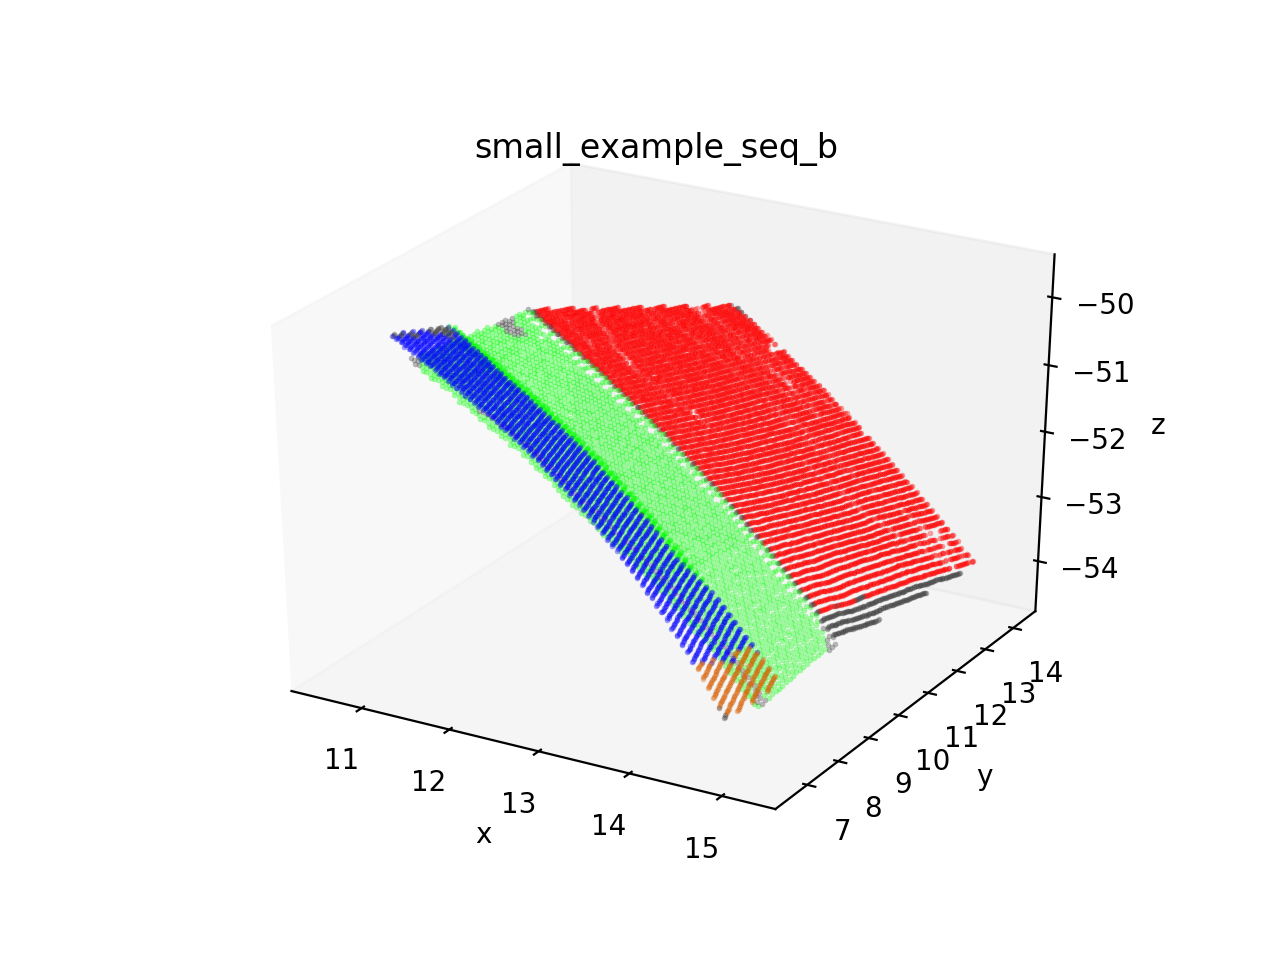
\includegraphics[scale=0.99]{small_example_seq_b.png}
\end{center}
\caption{The 40 to 50 scan line of the point cloud of small example.}
 \label{fig:40_50_sml_origin}
 \end{figure}
 
 %{0: 81461, 1: 27167, 2: 21583, 3: 2715, 4: 1112})

 \end{document}